\documentclass[tikz,border=12pt]{standalone}
\usepackage{tikz}
\usepackage{amsmath}
\usetikzlibrary{positioning,arrows.meta}

%% ── colour palette ────────────────────────────────────────────────────────
\definecolor{cMol}  {RGB}{189,214,232}   % MolFormer        – steel blue
\definecolor{cBank} {RGB}{252,243,207}   % Memory bank      – light gold
\definecolor{cHop}  {RGB}{250,218,180}   % Hopfield         – amber
\definecolor{cCtx}  {RGB}{187,228,187}   % Entropy gate     – sage green
\definecolor{cEp}   {RGB}{213,190,232}   % Evidential gate  – lavender
\definecolor{cGCN}  {RGB}{220,223,228}   % Graph / GCN      – cool gray
\definecolor{cPred} {RGB}{248,198,192}   % NIG head         – rose
\definecolor{cNone} {RGB}{248,248,248}   % Absent           – near white
\definecolor{cTitle}{RGB}{41, 82,130}    % Method title     – dark blue
\definecolor{cSep}  {RGB}{200,205,210}   % Column separator

\begin{document}
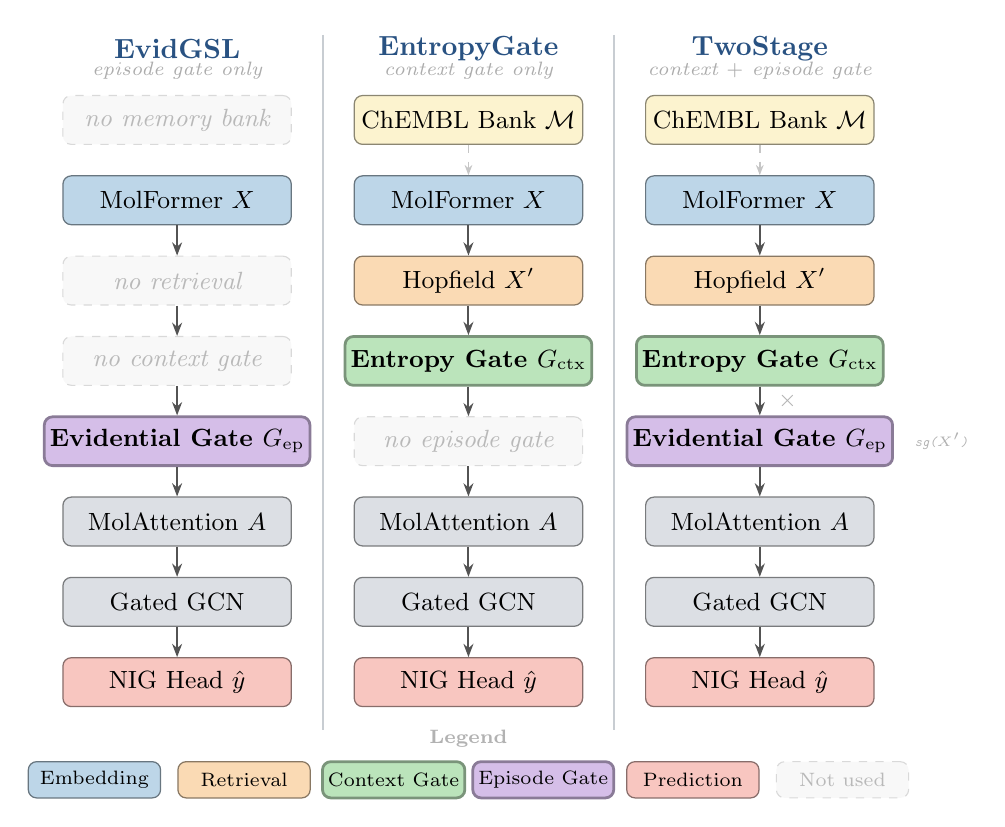
\begin{tikzpicture}[font=\small]

%% ── shared styles ─────────────────────────────────────────────────────────
\tikzset{
  blk/.style={
    rectangle, rounded corners=3pt,
    minimum width=2.90cm, minimum height=0.62cm,
    text centered, inner sep=2pt,
    draw=#1!55!black, fill=#1, line width=0.45pt
  },
  gate/.style={
    rectangle, rounded corners=3pt,
    minimum width=2.90cm, minimum height=0.62cm,
    text centered, inner sep=2pt, font=\small\bfseries,
    draw=#1!65!black, fill=#1, line width=1.0pt
  },
  absent/.style={
    rectangle, rounded corners=3pt,
    minimum width=2.90cm, minimum height=0.62cm,
    text centered, inner sep=2pt, font=\small\itshape,
    text=gray!55, draw=gray!30, fill=cNone, line width=0.4pt, dashed
  },
  arr/.style ={-{Stealth[scale=0.78]}, line width=0.70pt, gray!65!black},
  darr/.style={-{Stealth[scale=0.68]}, line width=0.55pt, gray!45, dashed},
}

%% ── column x-centres ──────────────────────────────────────────────────────
\def\cA{1.60}
\def\cB{5.30}
\def\cC{9.00}

%% ── row y-centres (shared grid) ───────────────────────────────────────────
%  row 0 : titles       y =  0.00
%  row 1 : bank         y = -0.90
%  row 2 : MolFormer    y = -1.92
%  row 3 : Hopfield     y = -2.94
%  row 4 : context gate y = -3.96
%  row 5 : episode gate y = -4.98
%  row 6 : MolAttention y = -6.00
%  row 7 : GCN          y = -7.02
%  row 8 : NIG head     y = -8.04

%% ══════════════════════════════════════════════════════════════════════════
%% COLUMN 1  –  EvidGSL
%% ══════════════════════════════════════════════════════════════════════════
\node[font=\normalsize\bfseries, text=cTitle]        at (\cA, 0.00)  {EvidGSL};
\node[font=\scriptsize\itshape,  text=gray!65]        at (\cA,-0.28)  {episode gate only};

\node[absent]              (A1R1) at (\cA,-0.90)  {no memory bank};
\node[blk=cMol]            (A1R2) at (\cA,-1.92)  {MolFormer $X$};
\node[absent]              (A1R3) at (\cA,-2.94)  {no retrieval};
\node[absent]              (A1R4) at (\cA,-3.96)  {no context gate};
\node[gate=cEp]            (A1R5) at (\cA,-4.98)  {Evidential Gate $G_{\mathrm{ep}}$};
\node[blk=cGCN]            (A1R6) at (\cA,-6.00)  {MolAttention $A$};
\node[blk=cGCN]            (A1R7) at (\cA,-7.02)  {Gated GCN};
\node[blk=cPred]           (A1R8) at (\cA,-8.04)  {NIG Head $\hat{y}$};

\draw[arr] (A1R2)--(A1R3);
\draw[arr] (A1R3)--(A1R4);
\draw[arr] (A1R4)--(A1R5);
\draw[arr] (A1R5)--(A1R6);
\draw[arr] (A1R6)--(A1R7);
\draw[arr] (A1R7)--(A1R8);

%% ══════════════════════════════════════════════════════════════════════════
%% COLUMN 2  –  EntropyGate
%% ══════════════════════════════════════════════════════════════════════════
\node[font=\normalsize\bfseries, text=cTitle]        at (\cB, 0.00)  {EntropyGate};
\node[font=\scriptsize\itshape,  text=gray!65]        at (\cB,-0.28)  {context gate only};

\node[blk=cBank]           (A2R1) at (\cB,-0.90)  {ChEMBL Bank $\mathcal{M}$};
\node[blk=cMol]            (A2R2) at (\cB,-1.92)  {MolFormer $X$};
\node[blk=cHop]            (A2R3) at (\cB,-2.94)  {Hopfield $X'$};
\node[gate=cCtx]           (A2R4) at (\cB,-3.96)  {Entropy Gate $G_{\mathrm{ctx}}$};
\node[absent]              (A2R5) at (\cB,-4.98)  {no episode gate};
\node[blk=cGCN]            (A2R6) at (\cB,-6.00)  {MolAttention $A$};
\node[blk=cGCN]            (A2R7) at (\cB,-7.02)  {Gated GCN};
\node[blk=cPred]           (A2R8) at (\cB,-8.04)  {NIG Head $\hat{y}$};

\draw[darr](A2R1)--(A2R2);
\draw[arr] (A2R2)--(A2R3);
\draw[arr] (A2R3)--(A2R4);
\draw[arr] (A2R4)--(A2R5);
\draw[arr] (A2R5)--(A2R6);
\draw[arr] (A2R6)--(A2R7);
\draw[arr] (A2R7)--(A2R8);

%% ══════════════════════════════════════════════════════════════════════════
%% COLUMN 3  –  TwoStage
%% ══════════════════════════════════════════════════════════════════════════
\node[font=\normalsize\bfseries, text=cTitle]        at (\cC, 0.00)  {TwoStage};
\node[font=\scriptsize\itshape,  text=gray!65]        at (\cC,-0.28)  {context $+$ episode gate};

\node[blk=cBank]           (A3R1) at (\cC,-0.90)  {ChEMBL Bank $\mathcal{M}$};
\node[blk=cMol]            (A3R2) at (\cC,-1.92)  {MolFormer $X$};
\node[blk=cHop]            (A3R3) at (\cC,-2.94)  {Hopfield $X'$};
\node[gate=cCtx]           (A3R4) at (\cC,-3.96)  {Entropy Gate $G_{\mathrm{ctx}}$};
\node[gate=cEp]            (A3R5) at (\cC,-4.98)  {Evidential Gate $G_{\mathrm{ep}}$};
\node[blk=cGCN]            (A3R6) at (\cC,-6.00)  {MolAttention $A$};
\node[blk=cGCN]            (A3R7) at (\cC,-7.02)  {Gated GCN};
\node[blk=cPred]           (A3R8) at (\cC,-8.04)  {NIG Head $\hat{y}$};

\draw[darr](A3R1)--(A3R2);
\draw[arr] (A3R2)--(A3R3);
\draw[arr] (A3R3)--(A3R4);
\draw[arr] (A3R4)--(A3R5)
           node[midway, right=3pt, font=\footnotesize, text=gray!60]{$\times$};
\draw[arr] (A3R5)--(A3R6);
\draw[arr] (A3R6)--(A3R7);
\draw[arr] (A3R7)--(A3R8);

% stop-gradient annotation
\node[font=\tiny\itshape, text=gray!60, right=4pt of A3R5]
  {\texttt{sg($X'$)}};

%% ── column separators ─────────────────────────────────────────────────────
\draw[cSep, line width=0.55pt] (3.45, 0.18) -- (3.45,-8.65);
\draw[cSep, line width=0.55pt] (7.15, 0.18) -- (7.15,-8.65);

%% ── legend ────────────────────────────────────────────────────────────────
\def\ly{-8.98}
\def\lw{1.68cm}
\def\lh{0.46cm}
\def\lfs{\scriptsize}

\node[font=\scriptsize\bfseries, text=gray!60] at (5.30,\ly+0.22) {Legend};

\node[blk=cMol,  minimum width=\lw, minimum height=\lh, font=\lfs]
  at (0.55,\ly-0.30) {Embedding};
\node[blk=cHop,  minimum width=\lw, minimum height=\lh, font=\lfs]
  at (2.45,\ly-0.30) {Retrieval};
\node[gate=cCtx, minimum width=\lw, minimum height=\lh, font=\lfs]
  at (4.35,\ly-0.30) {Context Gate};
\node[gate=cEp,  minimum width=\lw, minimum height=\lh, font=\lfs]
  at (6.25,\ly-0.30) {Episode Gate};
\node[blk=cPred, minimum width=\lw, minimum height=\lh, font=\lfs]
  at (8.15,\ly-0.30) {Prediction};
\node[absent,    minimum width=\lw, minimum height=\lh, font=\lfs]
  at (10.05,\ly-0.30) {Not used};

\end{tikzpicture}
\end{document}
